\documentclass{article}
\usepackage{authblk}
\usepackage{amsmath}
\usepackage{todonotes}
\usepackage{amssymb}
\usepackage{subcaption}
\usepackage[normalem]{ulem}
\usepackage{graphicx}
\usepackage{cite}
\usepackage{marginnote}
\usepackage[colorlinks=true,urlcolor=blue,citecolor=red,linkcolor=red,bookmarks=true]{hyperref}
\usepackage{soul}
\usepackage{pgfplots}
\pgfplotsset{compat=1.14}
\usepackage{tikz}
\usetikzlibrary{arrows.meta,shapes.geometric} 
\usepackage{float}
\usepackage{geometry}
\hypersetup{linkcolor=red,citecolor=green,urlcolor=blue}  


\newcommand{\fp}{P_{\text{fp}}}
\newcommand{\fn}{P_{\text{fn}}}
\newcommand{\Se}{S_\text{e}}
\newcommand{\Sp}{S_\text{p}}
\newcommand{\mi}{S_{\text{fn}}}
\newcommand{\err}[1]{E_{\text{{#1}}}}%_{\text{rel}}}
\newcommand{\eff}[1]{E_{\text{{#1}}}}%_{\text{rel}}}
\renewcommand\Affilfont{\itshape\small}
\renewcommand{\Pr}{\mathbb{P}}
\newcommand{\data}{\mathbf{d}}
\newcommand{\sens}{S_{\text{e}}}
\newcommand{\spec}{S_{\text{p}}}
% \newcommand{\tn}{P_{\text{tn}}}


\begin{document}
\title{An Accurate Model for SARS-CoV-2 pooled RT-PCR Test Errors}

\author[1,2]{Yair Daon, PhD}
\author[2,3]{Amit Huppert, PhD}
\author[1,2]{Uri Obolski, PhD}

\affil[1]{Porter School of the Environment and Earth Sciences, The
  Faculty of Exact Sciences, Tel Aviv University\\ Tel Aviv, Israel}

\affil[2]{School of Public Health, The Faculty of Medicine, Tel Aviv
  University\\ Tel Aviv, Israel}

\affil[3]{The Gertner Institute for Epidemiology and Health Policy
  Research, Tel Hashomer, Israel}
%\email{yair.daon@gmail.com}
\date{}

\maketitle

\begin{abstract}
\textbf{Background}: Pooling is a popular strategy for increasing
SARS-CoV-2 testing throughput. One popular pooling scheme is Dorfman
pooling: test $N$ individuals simultaneously. If the test is positive
--- retest each individual separately. However, requiring more than
one positive test may lead to increased false-negative rates.

\textbf{Methods}: We analyze the false-negative rate (i.e., the
probability of a negative result for an infected individual) of
Dorfman pooling via a new probabilistic model. We demonstrate that
different, previously made probabilistic assumptions regarding pooling
are unlikely in light of empiric data. Our model is conservative in
that it ignores sample dilution effects, which can only worsen pooling
performance.

\textbf{Results}: We show that one can expect a 60-80\% increase in
false-negative rates under Dorfman pooling, for reasonable parameter
values. Moreover, we show that the false-negative rates under Dorfman
pooling increase when the prevalence of infection decreases.

\textbf{Discussion}: In most pooling schemes, identifying an infected
individual requires positive results in multiple tests and hence
substantially increases false-negative rates. Furthermore, this
phenomenon is more pronounced when infection prevalence is low ---
exactly when pooling is most efficient. Thus, pooling presents an
inherent trade-off: it is most efficient when it is least
accurate. The deterioration of false-negative rates and the
aforementioned trade-off are inherent problems of pooling schemes and
should be kept in mind by practitioners and policy makers.
\end{abstract}

\section{Introduction}
Reverse transcription polymerase chain reaction (RT-PCR) testing is a
key component in breaking transmission chains and mitigating the
COVID-19 pandemic. As such, the need for large-scale testing has
resulted in the development of techniques to increase the the
throughput of RT-PCR tests \cite{DorfmanYuvalDor, PoolSize30,
  BayesianDorfman, MatrixPooling, LionDorfman}. These techniques,
often termed \emph{pooling}, or group testing, have originated in the
seminal work of Dorfman and his pooling technique
\cite{DorfmanOriginal, DorfmanYuvalDor}. Under Dorfman pooling, one
selects $N$ individuals and performs a single RT-PCR test on their
combined (\emph{pooled}) samples. If the pooled test yields a positive
result, then each individual is retested separately; otherwise,
everyone is declared negative. The throughput efficiency of Dorfman
pooling for has been demonstrated empirically \cite{DorfmanYuvalDor}
and its error rates thoroguhly investigated \cite{Kim, Simplistic1,
  OptimalDorfmanPool}.

Previous studies assumed that the probability of a true-positive (the
test's \emph{sensitivity}) does not depend on the number of infected
samples in the pool, but rather on the existence of at least one such
sample. Thus, the probability of a positive result in a pooled test
has been (assumed) identical for a pool with one sample from an
infected individual and, e.g., five such samples. This assumption is
common in the group testing literature \cite{Kim, OptimalDorfmanPool},
as well as in more specific, COVID-19 focused studies
\cite{Simplistic1, Simplistic2}. In this study we challenge these
commonly made assumptions and show how using a more accurate
probabilistic model affects estimation of false-negative rates for
Dorfman pooling.

\subsection{RT-PCR}\label{subsec:rtpcr}
We briefly explain the process of testing for SARS-CoV-2 by RT-PCR in
Section~\ref{subsec:rtpcr}. Our exposition intentionally avoids many
details, and a comprehensive review of RT-PCR can be found in
\cite{COVID-RTPCR, PCRBook}.

PCR is a process in which a targeted DNA strand's frequency is
amplified to create billions of copies in a reaction mixture. At the
end of this \emph{amplification} process, the presence of targeted DNA
molecules in a reaction mixture can be confidently
determined. Arguably, the best way to understand PCR is as a chain
reaction: Each targeted DNA molecule is copied into two, that are
copied into four and so forth. This cascade gives PCR its name:
polymerase chain reaction.

Specifically, the PCR process is comprised of cycles, with each cycle
doubling the abundance of the targeted DNA. In each cycle, each
double-strand DNA molecule is broken into two separate strands. An
enzyme called DNA polymerase generates a new double-strand DNA replica
from each separate strand. Replication cannot start without a specific
short DNA sequence, called a primer, that has to be introduced into
the reaction mixture. Introducing the right primer into the reaction
mixture ensures (almost) only the targeted DNA sequence is copied. A
protein is added to the reaction mixture, which emits light upon
successfully binding the targeted DNA. Once enough light is emitted
the tested reaction mixture is declared positive and a
\emph{detection} is said to occur. If, on the other hand, a predefined
number of cycles pass without a detection event then the reaction
mixture is declared negative.

Since the genetic material of SARS-CoV-2 is RNA rather than DNA, an
extra preprocessing step is required. An enzyme called reverse
transcriptase (hence the RT in RT-PCR) replicates existing RNA in the
reaction mixture into DNA. Once DNA replicas are made, the PCR process
proceeds as described above, targeting SARS-CoV-2 DNA replicas.

\subsection{Pooling}
One possible source of failed detection of SARS-CoV-2 RNA in pooled
RT-PCR testing (a \emph{false-negative}) is sample dilution. When
pooling, several samples are mixed, so the concentration of viral RNA
is reduced. This effect may cause a delay in amplification
\cite{DorfmanYuvalDor}, no detection and, consequently, a
false-negative. Another potential source for false-negatives is a
failed sampling process. 

%% However, \cite{Lion} showed that this effect can be
%% safely ignored when mixing up to 32 samples, which we correspondingly
%% assume.


\section{Methods}
We present the \emph{common assumption} in Section~\ref{subsec:common}
and refute it in Section~\ref{subsec:refute}. Our model is presented
in Section~\ref{subsec:ours}.

Formally, we consider a pool containing $N$ individuals
$\{1,\dots,N\}$. We denote the true infection states $\theta \in
\{0,1\}^N$, so individual $i$ is infected iff $\theta_i=1$. The RT-PCR
test's sensitivity (true-negative rate) is denoted $\sens$, and the
test's specificity (true-positive rate) is denoted $\spec$. Pooled
test result (data) is denoted $\data$, where $\data=0$ iff the test
returned a negative result.

\subsection{The common assumption}\label{subsec:common}
Previous studies of group testing strategies assumed that the
false-negative probability does not depend on the number of infected
samples, but merely on the existence of at least one such sample in a
pool \cite{Kim, OptimalDorfmanPool}. Current studies of pooling in the
context of SARS-CoV-2 also employ similar assumptions
\cite{Simplistic1, Simplistic2}. Specifically, these studies assume
that the probability of a negative result is the same for a pool with
a single sample coming from an infected individual and several
 samples from infected individuals. Explicitly:

\begin{align}\label{eq:common}
  \Pr(\data=0|\theta) = 
  \begin{cases} 
    1-\sens & \exists i\ \text{such that } \theta_i = 1\\
    \spec & \text{otherwise}
  \end{cases} 
\end{align}

Below, we refer to \eqref{eq:common} as the \emph{common
  assumption}. The essence of the common assumption is that
amplification takes place for all samples at once.
%% We refute the assumptions underlying \eqref{eq:common} in
%% Section~\ref{subsec:ours} and suggest more plausible ones in
%% Section~\ref{subsec:ours}.


\subsection{Refuting common assumption}\label{subsec:refute}
We refute the common assumption with experimental data summarized in
Table \ref{table}, collected from \cite{Salazar}. There, the authors
investigate Dorfman pooling and, regardless of the pooled test result,
follow up and test each pool member separately. We focus on 128 pools
for which at least one subsequent separate test was positive --- of
which 29 pooled tests were negative and 99 positive. In the data cited
in \cite{Salazar}, of the 29 negative pools, subsequent separate
testing yielded a single positive result in 24. In contrast, of the 99
positive pools, 42 yielded a single positive test upon subsequent
separate testing.

The data in Table \ref{table} allows us to test the following null
hypothesis $H_0$: The probability of a pooled false-negative is equal
for pools with one subsequent positively tested member and pools with
two or more such members. $H_0$ is a direct consequence of the
assumptions, and rejecting $H_0$ implies the common assumption are not
realistic, at least for SARS-CoV-2.

We apply Fisher's exact test for the presence of more than one
positive individual in correctly identified pools. Fisher's test
yields an increased odds ratio of 6.4, 95\% CI (2.2,23.4), with a
p-value $\approx 10^{-4}$. Thus, we reject $H_0$, refuting the common
assumption.

\begin{table}[h]
\centering
\begin{tabular}{ c c c }
                                & Negative pool  & Positive pool \\%& Row total \\ 
\# subsequent positives $=1$    & 24             & 42            \\%& 66        \\  
\# subsequent positives $\geq1$ & 5              & 57            \\%& 62        \\
 Total                          & 29             & 99            \\%& 128 
\end{tabular}
\caption{Contingency table of data from \cite{Salazar}}\label{table}
\end{table}

\subsection{Our model}
Since the essence of the failed common assumption is that
amplification of all samples occurs only once, we assume the opposite:
amplification of viral RNA occurs for each sample independently.
According to \cite{Simplistic1, Simplistic2, Kim, OptimalDorfmanPool},
erroneous detection (a false-positive) does not depend on the number
of negative samples in a pool. We incorporate this assumption in our
model with a small modification: We assume that an erroneous
amplification can occur in \emph{any} pool. Specifically, it is
possible that correct amplifications fail and an erroneous one occurs
simultaneously. This assumption is somewhat specific for the current
application of screening for SARS-CoV-2 via RT-PCR. For example,
cross-reactivity with other coronaviruses would have violated this
assumption, but it was ruled out in \cite{KitComparison}.

\begin{figure}[H]
  \centering
  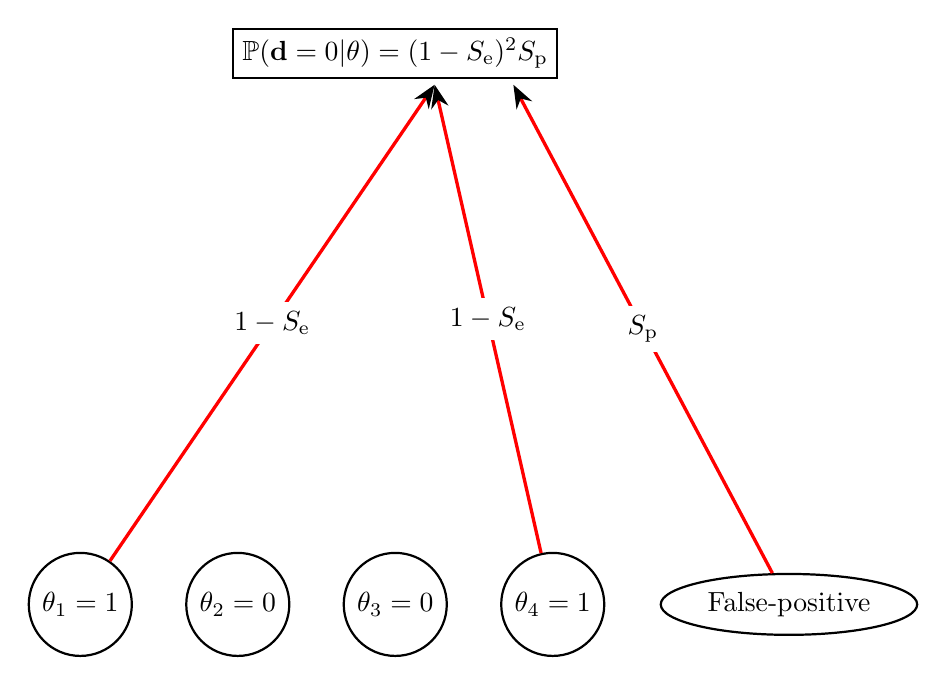
\begin{tikzpicture}
    \begin{scope}[every node/.style={circle,thick,draw}]
      \node[shape=circle,draw=black] (A) at (0,0) {$\theta_1=1$};
      \node[shape=circle,draw=black] (B) at (2,0) {$\theta_2=0$};
      \node[shape=circle,draw=black] (D) at (4,0) {$\theta_3=0$};
      \node[shape=circle,draw=black] (E) at (6,0) {$\theta_4=1$};

      \node[shape=ellipse,draw=black]
      (F) at (9,0) {False-positive};
      
      \node[shape=rectangle,draw=black] (G) at (4,7)
           {$\Pr(\data=0|\theta)=(1-\sens)^2\spec$};
    \end{scope}

    \begin{scope}[>={Stealth[black]},
        every node/.style={fill=white},
        every edge/.style={draw=red,very thick}]
      \path [->] (A) edge node {$1-\sens$} (4.5,6.6);
      %\path [->] (B) edge node {$0$} (G);
      %\path [->] (D) edge node {$0$} (G);
      \path [->] (E) edge node {$1-\sens$} (4.5,6.6);
      \path [->] (F) edge node {$\spec$} (5.5,6.6); 
    \end{scope}
  \end{tikzpicture}
  \caption{Illustration of our model. A pool contains individuals
    $\{1,2,3,4\}$ with state $\theta=(1,0,0,1)$ (i.e. individuals 1
    and 4 are infected). A negative pooled test ($\data=0$) implies
    that three detection paths failed. A false-negative occurred for
    $1$ and $4$, each with probability $(1-\sens)$ for
    each. Additionally, no erroneous detection of SARS-CoV-2 occurred,
    with probability $\spec$. Individuals $2$ and $3$ are not infected
    and do not contribute to the probability of the pooled test
    result. A positive pooled test arises if any one of the above
    mentioned paths results in a detection.}\label{fig:likelihood}
\end{figure}

To summarize, we assume that for a single pool, a positive test result
is generated in one of two paths. Either, SARS-CoV-2 RNA from an
infected individual's sample is correctly amplified and detected, and
this can happen for each positive sample in a pool, with probability
$\Se$. Or, some erroneous amplification occurs (e.g. contaminant viral
RNA is introduced), an event that occurs at most once per pool, with
probability $1-\Sp$. Our model is illustrated in
Figure~\ref{fig:likelihood}, and summarized in
%% A negative pooled test result occurs when all detection paths (both
%% correct and erroneous) fail. The probability of no false-detection
%% accounts for the $\spec$ term. The probability of no correct detection
%% is $(1-\sens)$ per infected individual. The probability that all such
%% paths fail is the product of the above mentioned terms, displayed in
\eqref{eq:likelihood a}.%%  The probability of a positive result,
%% presented in \eqref{eq:likelihood b}, is simply the complement.
%% The probability of a negative pooled test result is presented in
%% \eqref{eq:likelihood a} (along with its complement
%% \eqref{eq:likelihood b}), and explained below.
%\begin{subequations}
\begin{align}%\label{eq:single likelihood}
  %\begin{split}
    \Pr(\data=0 | \theta) &= \spec\prod_{i=1}^N
    (1-\sens)^{\theta_i} = \spec(1-\Se)^{\sum_i\theta_i}. \label{eq:likelihood a}
    %
    %
    %
    %% \Pr(\data=1 | \theta) &= 1 - \spec\prod_{i=1}^N
    %% (1-\sens)^{\theta_i} = 1 - \spec(1-\Se)^{\sum\theta_i} . \label{eq:likelihood b}
  %\end{split}
\end{align}
%\end{subequations}
%% Combining \eqref{eq:likelihood a} and \eqref{eq:likelihood b}, and
%% recalling that $\data \in \{0,1\}$ yields:

%% \begin{align}\label{eq:combined likelihood}
%%   \begin{split}
%%     \Pr(\data| \theta) &= \left [\spec\prod_{i=1}^N
%%       (1-\sens)^{\theta_i} \right ]^{1-\data} \left [1 - \spec\prod_{i=1}^N (1-\sens)^{\theta_i} \right ]^{\data}.
%%   \end{split}
%% \end{align}


\subsection{Application}
As an application of our model, we calculate the differnece in
false-negative rate for a single \emph{infected} individual,
henceforth referred to as "Donald". We distinguish three types of
false-negative events when performing pooling. A \emph{single test}'s
false-negative is the event of a negative result upon testing Donald
separately, i.e., in an RT-PCR test without pooling. A \emph{pooled}
false-negative occurs when a pooled test containing Donald's sample
(and other samples) yields a negative result, i.e., the pooling fails
to detect at least one positive result. Lastly, a \emph{scheme}
false-negative occurs when an entire pooling scheme fails to identify
Donald as infected. Our goal is to calculate Dorfman's scheme
false-negative rate. Rephrasing, we wish to answer the following
question: what is the probability of not identifying Donald as
infected under a Dorfman pooling scheme?

\subsubsection{Scheme false-negative rate}
Denote the prevalence of infection in the (tested) population $q$. We
give Donald the respect he deserves and assign him as individual $1$,
so that $\theta_1=1$. Then:

\begin{align}
  \begin{split}
    \Pr(\data=0|\theta_1=1) &= \sum_{\theta_2,\dots,\theta_N}
    \Pr(\theta_2,\dots,\theta_N)
    \Pr(\data=0|\theta_1=1,\theta_2,\dots,\theta_N) \\
    %
    %
    %
    &= \sum_{k=0}^{N-1}\Pr(\sum_{i=2}^N\theta_i=k)
    \Pr(\data=0|\theta_1=1,\sum_{i=2}^N\theta_i = k)\\
    %
    %
    %
    &= \sum_{k=0}^{N-1}\binom{N-1}{k}q^k(1-q)^{N-1-k} \Sp(1-\Se)^{1+k}\\
    %
    %
    %
    &= \Sp(1-\Se) \sum_{k=0}^{N-1}\binom{N-1}{k}
    \left(q(1-\Se)\right)^k(1-q)^{N-1-k}\\
    %
    %
    %
    &= \Sp(1-\Se)(1-q\Se)^{N-1}, \text{ by Newton's Binomial Theorem.} \\
  \end{split}
\end{align}

If the pooled test yields a positive result, Donald is tested
separately. Taking a conservative stand, we assume such a simple
procedure poses no risk of introducing contaminant RNA. Therefore, the
separate test yields a positive result with probability $\Se$.

We calculate the probability that Donald is mistakenly identified as
not infected, henceforth referred to as the scheme's false-negative
rate and denoted $\mi$. In order to correctly identify Donald
as infected, both pooled and separate tests have to yield a positive
result. Thus, the scheme's false-negative rate is:
\begin{align}\label{eq:sfn}
    \begin{split}
        \mi :&= 1 - \Se\Pr(\data=1|\theta=1)\\
        %
        &= 1 - \Se\left [1 - \Sp(1-\Se)(1-q\Se))^{N-1}\right].
    \end{split}
\end{align}

\subsubsection{Comparison metric}
The single test false-negative rate $1-\Se$ and scheme false-negative
rate $\mi$ are compared via:
\begin{equation}\label{eq:erel}
\rel{ours} := \frac{\mi - (1-\Se)}{1-\Se} \cdot 100.
\end{equation}
$\rel{ours}$ is the percentage increase in the pooling scheme false-negative
rate, relative to the single test false-negative rate.

According to the common assumption, the scheme false-negative rate is
$1-\Se^2$. A short calculation shows that this approximation implies
the percentage increase in scheme false-negative rate is just
$\rel{common} := 100\cdot \Se$.

\section{Results}\label{section:results}
We plot $\rel{ours}$ for varying prevalence $q$ and sensitivity $\Se$
values, and make the comparison with $\rel{common}$. As recommended by
\cite{DorfmanYuvalDor}, we apply different pool sizes $N$, for
different prevalence values. We observe that for a false-positive rate
$\Sp=0.95$ \cite{DorfmanYuvalDor} and a range of reasonable
sensitivity and prevalence values \cite{KitComparison,
  InterpretingCOVID19Test, EstimatingRatesLourenco,
  FalsePositiveEstimate}, an increase of at least $60\%$ in
$\rel{ours}$ can be expected (Figure \ref{figy}).

Interestingly, an increase in infection prevalence monotonically
decreases the scheme false-negative rate, as can also be easily seen
from \eqref{eq:sfn}. For the chosen parameter ranges, the increase in
the single test false-negative rates increases the relative error
$\rel{ours}$. These effects can be seen in Figure \ref{figy} (left
panel), upon conditioning on pool size. Extending the range for $\Sp$
yields no qualitative differences. We further compare $\rel{ours}$ to
$\rel{common}$, showing the discrepancy changes as a function of both
prevalence and the single test sensitivity (Figure \ref{figy}, right
panel).
\begin{figure}[H]
  \centering
  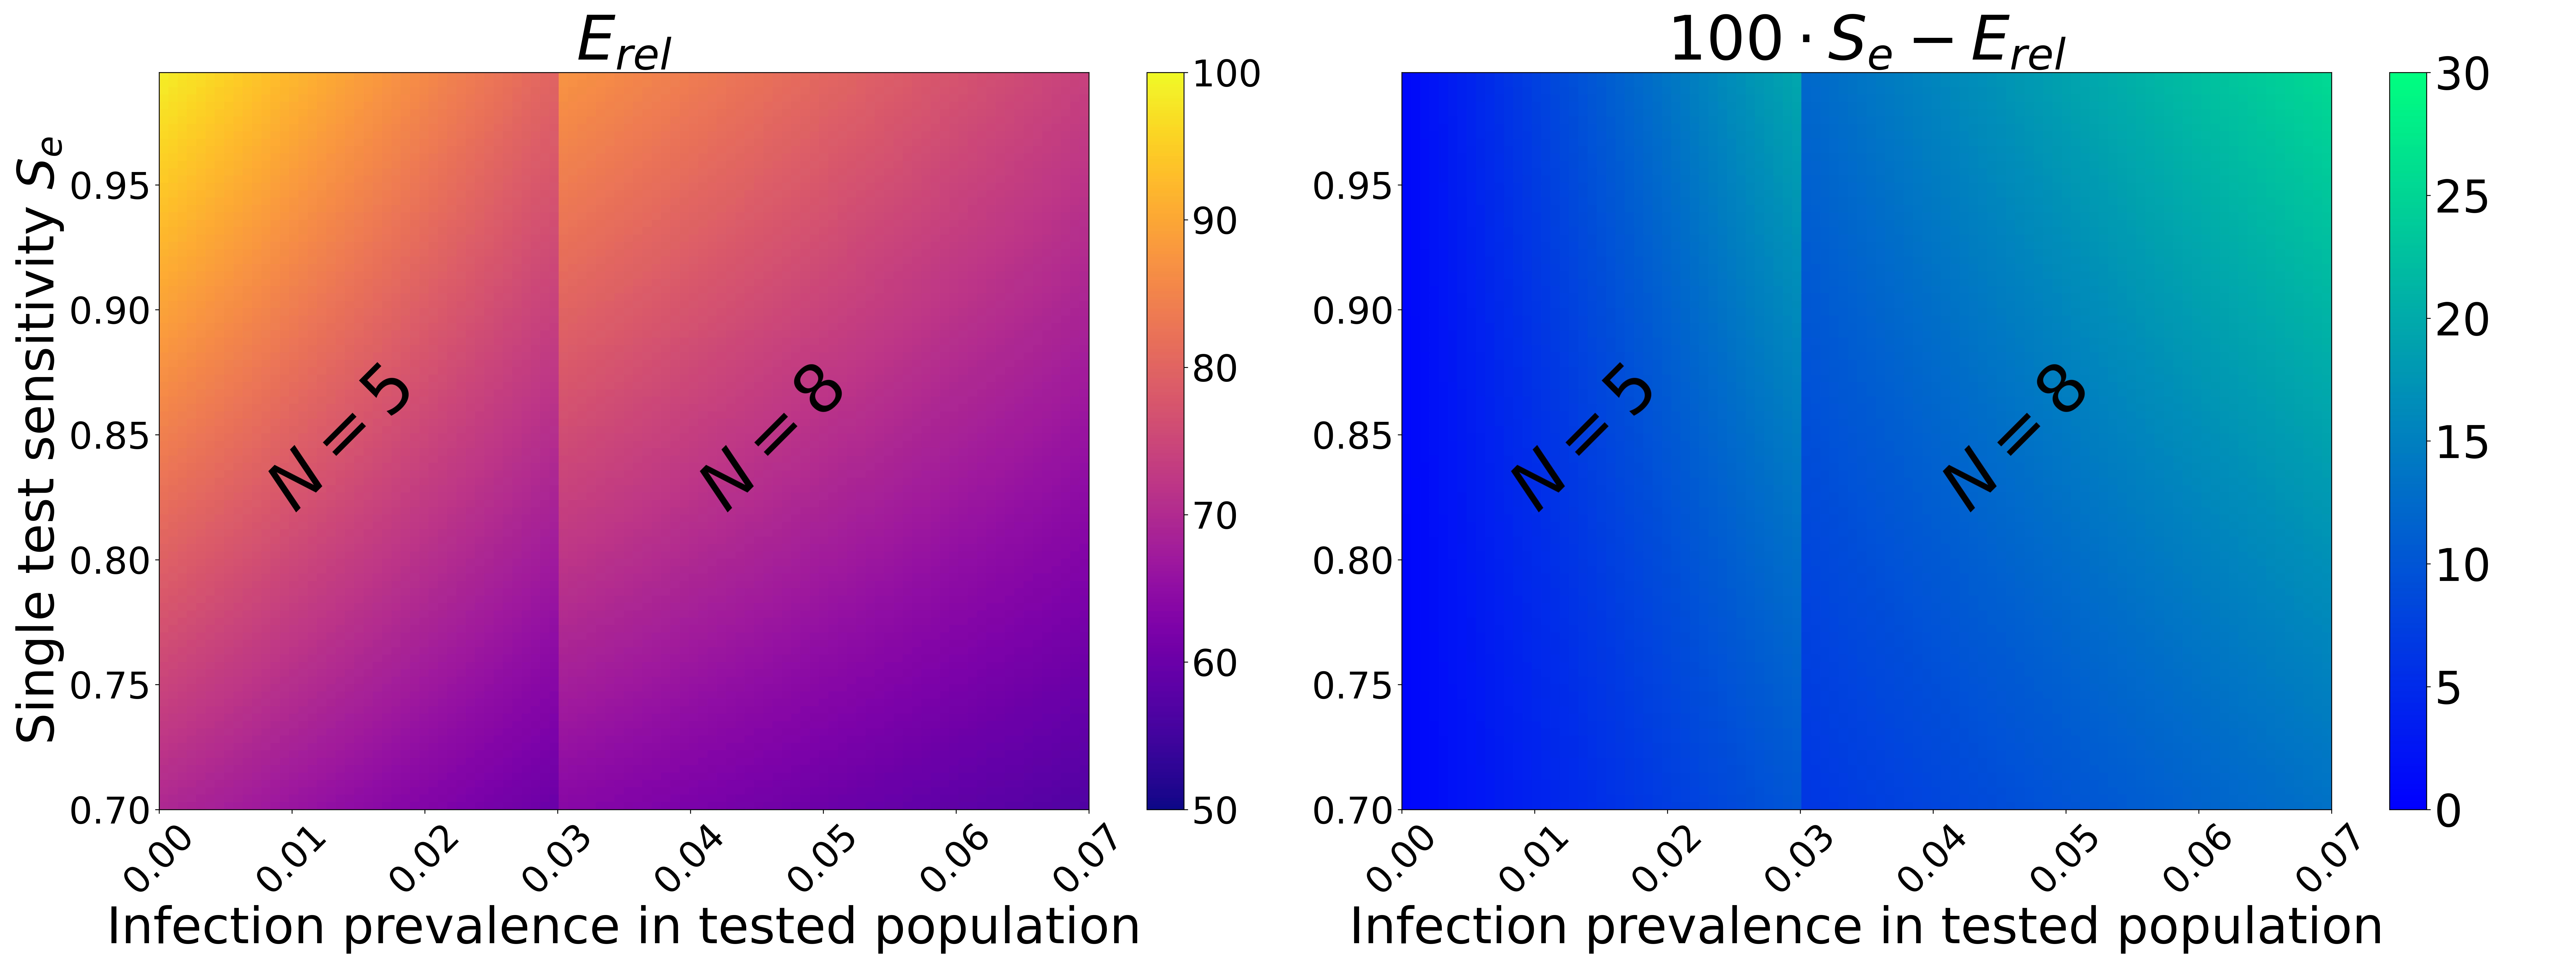
\includegraphics[width=18cm]{heatmap.jpg}
  \caption{Relative increase in Dorfman pooling false-negative rates
    $\rel{ours}$. Left: Colors represent $\rel{ours}$, the relative
    percentage increase in the scheme false-negative rates relative
    to the single test false-negative rates (eq
    \eqref{eq:erel}). Right: colors represent the difference between
    $\rel{common}$ and $\rel{ours}$. The disease prevalence $q$, is
    varied on the x-axis, while the test sensitivity is varied on
    the y-axis. Pool size $N$, was chosen according to $q$ as in
    \cite{DorfmanYuvalDor}.}\label{figy}
\end{figure}


\section{Discussion}
We have presented a novel model for pooled tests. It is hard to
assess the validity of our model, since this would require
considerably more data than available in \cite{Salazar}. However, our
model is as simple as possible, given that the standard assumptions
are refuted. We have no doubt that further study of the assumptions
underlying pooling is due. Furthermore, adapting common group testing
algorithms \cite{Kim} to novel error models should be further
studied.

Our revised model has some implications for the practice of
pooling. For example, although Dorfman pooling improves testing
throughput, we have shown that low values of infection prevalence, or
low values of single test false-negative rates, increase
$\rel{ours}$. These results remain qualitatively similar under varying
parameter values, in the observed ranges
\cite{KitComparison,EstimatingRatesKucrika, EstimatingRatesLourenco,
  InterpretingCOVID19Test} (Figure \ref{figy}).

Our results lead to a fact almost disregarded in
\cite{DorfmanYuvalDor}: although (Dorfman) pooling is most efficient
when prevalence is low, such circumstances are exactly those leading
to a substantial increase in false-negative rates. Such behavior of
pooling is not implied by the common assumption


%% The common assumption implies that one assumes that the probability of
%% a false-negative is identical for the pooled and single
%% tests. Although simplistic in nature, the common assumption does capture
%% the intuition behind our results: For Donald to be considered negative
%% under Dorfman pooling, he has to test negative twice. In addition to
%% this approximation only being an upper bound \cite{Simplistic2}, it
%% does not account for the effect of infection prevalence on the
%% false-negative rates under Dorfman pooling. Supporting the importance
%% of this effect, such an association between prevalence and the scheme
%% false-negative rate under Dorfman pooling has been empirically noted
%% \cite{DorfmanYuvalDor}.

Although our application focused on Dorfman pooling, our analysis
applies to other pooling schemes. Pooling schemes
(e.g. \cite{MatrixPooling,Lion, Kim}), require some sequence of
positive pooled results to correctly identify Donald as
infected. Consider the hierarchical pooling scheme \cite{Lion, Kim}:
If the first pool yields a positive result, it is split in two. Then
the splitting is repeated until resulting pools are negative or
individuals are tested separately. With an initial pool size of 32,
Donald will necessarily have to test positive in pools of size 32, 16,
8, 4 and 2, as well as in a single test, for the scheme to correctly
identify him as infected. Compare this to the Dorfman scheme that
requires a positive test in a pool of size $N=8$, and an additional
single positive test to identify Donald as infected. The hierarchical
pooling scheme of \cite{Lion, Kim} will necessarily yield more
false-negatives than Dorfman pooling --- there are additional places
for it to fail.

As mentioned in \cite{DorfmanYuvalDor}, introducing a positive
dependence within a pool decreases the false-positive rate. In the
extreme case, consider a fully connected pool, where one infection
implies the entire pool is infected. In this case, a calculation
analogous to the one conducted above recovers the initial
false-negative rate $1-\Se$. Interestingly, pooling was also noted to
have increased throughput when infection probabilities are dependent
between the pooled individuals \cite{DorfmanYuvalDor}, providing
another advantage to sampling dependent individuals in pooling
schemes.

To conclude, pooling is an important technique which can improve
testing throughput in a cost-effective manner. Nevertheless, a
substantial increase in pooling schemes' false-negative rates can be
expected. Such an increase has crucial implications for controlling
the spread of COVID-19.




\bibliographystyle{amsplain}
%\bibliographystyle{ama}
\bibliography{refs}

\end{document}
